\section{Formulation}\label{sec:formulation}
\subsection{System modeling}
The dynamics of a general floating-base system can be written as
\begin{equation}\label{eq:rigid_body_dyn}
B(q)\,\dot{v} +C(q, v)\,v + g(q) = \tau_{a} + J^T\,f
\end{equation}
where $B\in\mathbb{R}^{n_v\times n_v}$ and $C\in\mathbb{R}^{n_v\times n_v}$ are, respectively, the generalized inertia and Coriolis matrices of the system; $q\in\mathbb{R}^{n_q}$ and $v\in\mathbb{R}^{n_v}$ are the configuration and generalized velocity vectors of the system, while $g\in\mathbb{R}^{n_v}$ and $\tau_a=\begin{bmatrix}
0_{6\times 1};
\tau_{\mathrm{m}}
\end{bmatrix}\in\mathbb{R}^{n_v}$ are, respectively, the generalized gravity vector and the actuation torques. Finally, $J^T(q)\,f$ are the torques generated by the generalize wrench $f$ through the contact jacobian $J$. In the specific case of our leg prototype, the system has a degenerate floating base with only a single degree of freedom, given by the sliding guide joint (see Fig.~\ref{fig:jumping_sequence}); as a consequence, $\tau_a$ is simply $\begin{bmatrix}
0;\,\tau_{\mathrm{m}}\end{bmatrix}$, $n_q = n_v = 3$, $J\in\mathbb{R}^{3\times 3}$ and $f\in\mathbb{R}^3$, if we only consider a point contact with the ground.
\subsection{Actuator modeling: quadrature current estimation}
% As already highlighted in Sections~\ref{sec:introduction} and ~\ref{sec:prb_def}, jumping motions are particularly demanding for the robot. In particular, the high torques required to perform the take-off and to stop the robot after the impact have to be produced by the Brushless Direct Current (BLDC) actuators of the leg. 
It is known~\cite{foc::krause2013analysis} that the torque-quadrature current characteristic for Brushless Direct Current (BLDC) actuators is well approximated by the relationship
\begin{equation}\label{eq:torque_iq}
\tau_m = K_t\,i_q
\end{equation}
with the $K_t\in\mathbb{R}$ is the torque constant of the motors.
% Hence, high driving torques need to be produced by high quadrature currents. This two quantities cannot assume, however, arbitrarily large values, due to both mechanical and electrical limitations. Even if our prototype is equipped with current (and torque) sensors, in order to preemptively avoid damage to the hardware, it is also crucial to embed an estimate model of the actuators into our TO formulations.
% We start by writing the motor-side dynamics for a single actuator as in~\cite{friction_comp::le2008friction}:
% \begin{equation}\label{eq:rotor_dyn}
%     \tau_m + \tau_r = I_r\,\dot{v}_m
% \end{equation}
% where $\tau_m$ is the driving torque acting on the rotor, $\tau_r$ includes all torques coming from the reduction stage of the actuator. $I_r$ is the rotational inertia of the rotor and $\dot{v}_m$ is acceleration of the rotor. If no losses are present between the robot and the link side, $\tau_r$ is simply equal to the torques measured at the link, reflected to the motor (through the reduction ratio). However, when working with non direct-drive actuators, there will always be an amount of losses in the reduction stage. This was especially true in our case, where the actuators posses a reduction ratio of $1:50$ and there is a relevant amount of friction at the joints.
Employing this information, we can write a friction-compensated version of the rotor-side dynamics as in~\cite{friction_comp::le2008friction}:
\begin{equation}\label{eq:rotor_dyn_friction}
    K_t\,i_q  - \tau_l\,\eta + 
\tau_{\mathrm{fl}} \, \eta = I_r\,\dfrac{\dot{v}_l}{\eta}
\end{equation}
where $\tau_l\in\mathbb{R}^{2}$ are the link side torques acting on the actuators, $\tau_{\mathrm{fl}}\in\mathbb{R}^{2}$ is a vector modeling the friction torques reflected at the link-side, $i_q\in\mathbb{R}^{2}$ are the quadrature currents, $0 < \eta \leq 1$ is the reduction ratio from the motor to link side and $I_r$ is the axial inertial of the rotor. Equation~\eqref{eq:rotor_dyn_friction} can be used to build a friction observer (as done in~\cite{friction_comp::le2008friction}) or, alternatively, can be employed to calibrate a suitable friction model for $\tau_{\mathrm{fl}}$.
% The availability of such a model, as already highlighted, will be crucial in enforcing realistic constraints into our TO formulation. 
Specifically, we use the simple Coulomb-like friction model 
\begin{equation} \label{eq:friction_torque}
\tau_{\mathrm{fl}} = - K_{\mathrm{f, s}}\,\mathrm{signh}({v_l}) - K_{\mathrm{f, d}}\,v_l
\end{equation}
where $\mathrm{signh}()$ is a smooth approximation of the sign function based on the hyperbolic tangent and the scalars $K_{\mathrm{f, s}}$ and $K_{\mathrm{f, d}}$ are the static and dynamic friction coefficients respectively. We employ~\eqref{eq:rotor_dyn_friction} to estimate the friction coefficients in~\eqref{eq:friction_torque} by solving a simple least-squares regression problem with data collected during suitable calibration trajectories. Figure~\ref{fig:iq_model_tracking} shows the tracking performance of the resulting calibrated model w.r.t. actual measurements.
\begin{figure}
    \centering
    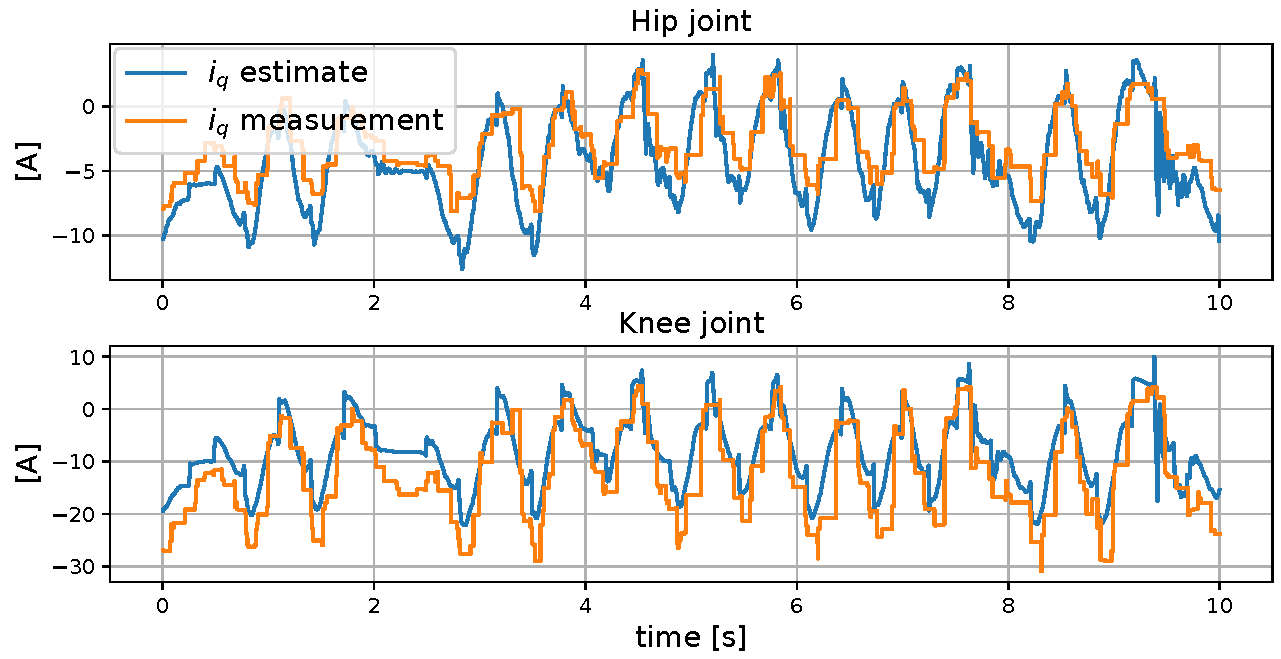
\includegraphics[width=1.0\columnwidth]{images/iq_tracking.pdf}
    \caption{Validation of the quadrature current $i_q$ model during a simple test: the leg stands on the ground with low-joint impedance and a vertical pushing force is applied to the base link. The tracking of the calibrated model is accurate, thus justifying its incorporation into our TO formulation.}
    \label{fig:iq_model_tracking}
\end{figure}
\subsection{Take-off optimization: maximizing the reached apex height}\label{subsec:takeoff_opt}
% \begin{figure}
%     \label{fig:ref_vs_res}
%     \centering
%     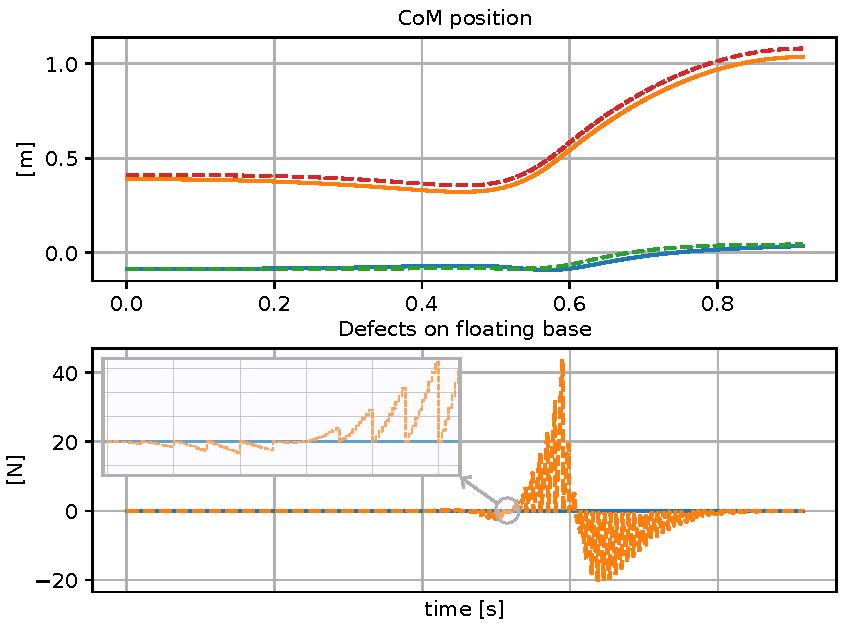
\includegraphics[width=1\columnwidth]{images/defects_full_with_zoom.pdf}
%     \caption{Importance of the refinement step for the take-off TO formulation. The re-sampled solution, shown as dotted lines, has relevant dynamic defects on the floating base (i.e. the sliding guide). The force on that joint should be $0$ for a feasible solution. On the contrary the solution of the refined problem has $0$ defects. Also, note how the CoM trajectory of the refined solution is different.}
% \end{figure}
Given the scope of our case study, we are interested in performing the jumping task with the highest performance our prototype is able to offer. For a jumping trajectory, this means maximizing the height at the apex of the jump, while accounting for the hardware's constraints. To achieve this, we employ an inverse dynamics-based formulation and hence use accelerations $\dot{v}$ and contact forces $f$ as inputs to the rigid body dynamics~\eqref{eq:rigid_body_dyn}. The benefits of employing inverse-dynamics based formulations, as opposed to forward-dynamics based ones, are starting to become apparent~\cite{to::ferrolho2021inverse},~\cite{to::mastalli2022inverse}: an increased numerical efficiency and stability, particularly for coarse discretizations. We define the states and inputs vectors $x_t$ and $u_t$ of  our take-off TO as
\begin{eqnarray}
&x_t = \left[q,~v,~\dot{v},~f\right]\label{eq:states_takeoff_opt}\\
&u_t = \left[\ddot{v},~\dot{f}\right]\label{eq:inputs_takeoff_opt}
\end{eqnarray}
The running cost of the TO is formulated as
\begin{dmath}\label{eq:takeoff_running_cost}
    \ell_{t}(x_t,~u_t) = \ell_f + \ell_{\dot{f}} + \ell_{v} +  \ell_{\dot{v}} + \ell_{\ddot{v}}
\end{dmath}
where the weighted costs $\ell_{f}$, $\ell_{\dot{f}}$, $\ell_{v}$, $\ell_{\dot{v}}$, $\ell_{\ddot{v}}$ are all quadratic in, respectively, $f$, the yank $\dot{f}$, $v$, $\dot{v}$ and the jerk $\ddot{v}$. 
The cost for the maximization of the CoM height $h_{\mathrm{CoM}}$ is implemented as a terminal constraint at the apex time $T_{\mathrm{apex}}$ of the form 
\begin{equation}\label{eq:max_com}
\ell_{\mathrm{CoM}}^F(T_{\mathrm{apex}}) = \dfrac{1}{h_{CoM}(q(T_{\mathrm{apex}})) + \epsilon}
\end{equation}
where $\epsilon$ is a small positive number to avoid singularities.
The only non-linear cost is the term $\ell_{\mathrm{CoM}}$, which maximizes the height of the CoM. The integral cost of the take-off TO can hence be written as
\begin{dmath}\label{eq:takeoff_opt_L}
    L_{t} \left( W_t\right) = \ell_{\mathrm{CoM}}^F + \int_{0}^{T_{\mathrm{apex}}}\,\ell_{t}(\tau)\,d\tau
\end{dmath}
where
\begin{equation}\label{takeoff_opt:opt_vars}
W_t \coloneqq \left[x_t,~u_t,~T_{\mathrm{takeoff}},~T_{\mathrm{apex}}\right]
\end{equation} 
collects our optimization variables and $T_{\mathrm{takeoff}}$ and $T_{\mathrm{apex}}$ represent, respectively, the take-off and apex instant. 
The cost function~\eqref{eq:takeoff_opt_L} is complemented by a set constrains, which are used to  enforce both the jumping maneuver and a series of crucial hardware constraints. First, defining $\tau_{\mathrm{lim}}$ as the actuated joints torque limits, we impose bounds on the torques $\tau_a$:
\begin{equation}\label{eq:tau_lims}
- \begin{bmatrix}
0\\
\tau_{\mathrm{lim}}
\end{bmatrix} \leq \tau_a \leq \begin{bmatrix}
0\\
\tau_{\mathrm{lim}}
\end{bmatrix}
\end{equation}
Furthermore we constrain the tip to stay on the ground before the takeoff instant with the following couple of constraints, respectively, on the tip position $\chi_{\mathrm{tip}}$ and velocity $\dot{\chi}_{\mathrm{tip}}$
\begin{eqnarray}
&\chi_{\mathrm{tip, z}} = 0 \label{eq:tip_on_ground}\label{eq:tip_on_ground_vel};~t = 0\\
&\dot{\chi}_{\mathrm{tip}} = 0;~t\in\left[0, T_{\mathrm{takeoff}}\right]
\end{eqnarray}
We also impose the apex at the final instant with the terminal constraint
\begin{equation}\label{eq:apex_com}
\dot{\chi}_{\mathrm{CoM, z}} = 0;~t = T_{\mathrm{apex}}
\end{equation}
% The flight phase is imposed by constraining the contact force to be null after the takeoff, up to the final instant. Furthermore $f$ should always be positive and its tangential component $f$ should lie inside the friction pyramid defined by the coefficient~$\mu$ and the tangential an normal components $f_t$ and $f_n$. Summing up:
We impose contact and friction contraints on $f$ with
\begin{eqnarray}\label{eq:f_cnstrnt}
&f \geq 0;~t\in\left[0, T_{\mathrm{takeoff}}\right] \label{eq:f_positive} \\
&f = 0; ~t\in\left[T_{\mathrm{takeoff}}, T_{\mathrm{apex}}\right] \\
&-\mu\,f_n \leq f_t\leq \mu\,f_n;~t\in\left[0, T_{\mathrm{takeoff}}\right] 
\end{eqnarray}
At the first instant, the leg should also start still; as a consequence
\begin{equation}\label{eq:starts_still}
    v = 0;~t = 0
\end{equation}
We also account for the calibrated actuation model~\eqref{eq:rotor_dyn_friction} by constraining the quadrature current $i_q$ of the actuator as
\begin{eqnarray}
&K_t\,i_q  - \tau_{l}\,\eta + 
\tau_{\mathrm{fl}} \, \eta = I_r\,\dfrac{\dot{v}_l}{\eta}\label{eq:rotor_dyn_friction_cnstrnt}\\
&- i_{q, \mathrm{max}} \leq i_q \leq i_{q, \mathrm{max}}\label{eq:rotor_dyn_friction_cnstrnt2}
\end{eqnarray}
Finally, we can write the continuous version of our take-off TO as
\begin{subequations}\label{eq::takeoff_opt_prb}
	\begin{dmath}
		\min_{W_t}~L_{t}\left(W_t \right)
	\end{dmath}
	\centering\text{subject to}
	\begin{eqnarray}
	&\text{rigid body dynamics}~\eqref{eq:rigid_body_dyn}
    \label{eq:rigid_body_dyn_cnstrnt}\\
    &~\text{constraints}~\text{~\eqref{eq:tau_lims}~to~ \eqref{eq:rotor_dyn_friction_cnstrnt2}} \\
    &\text{joint position and velocity ranges}
	\end{eqnarray}
\end{subequations} 

The continuous TO problem described by~\ref{eq::takeoff_opt_prb} is then transcribed over a grid of $N$ nodes by employing the multiple shooting method~\cite{to::bock1984multiple}. The solution to the discretized version of~\eqref{eq::takeoff_opt_prb} is first re-sampled at a desired constant rate following the procedure detailed in~\cite{to::horizon_to} and then fed as initial guess to a \textit{refined} discretized problem with the same costs and constraints as~\eqref{eq::takeoff_opt_prb}, but with fixed time intervals. This procedure, very similar to the \enquote{mesh refinement} employed in~\cite{to::horizon_to}, is needed to make the re-sampled solution dynamically feasible. As shown in~\cite{to::horizon_to}, in fact, the re-sampling procedure may introduce large dynamics defects on the floating-base of the robot, thus making the obtained solution dynamically unfeasible. 
As an additional remark, the authors would like to underline the importance of the terms $\ell_{\dot{f}}$ and $\ell_{\ddot{v}}$ in minimizing the feasibility gap between simulation and reality.
\begin{figure}[t]
    \centering
    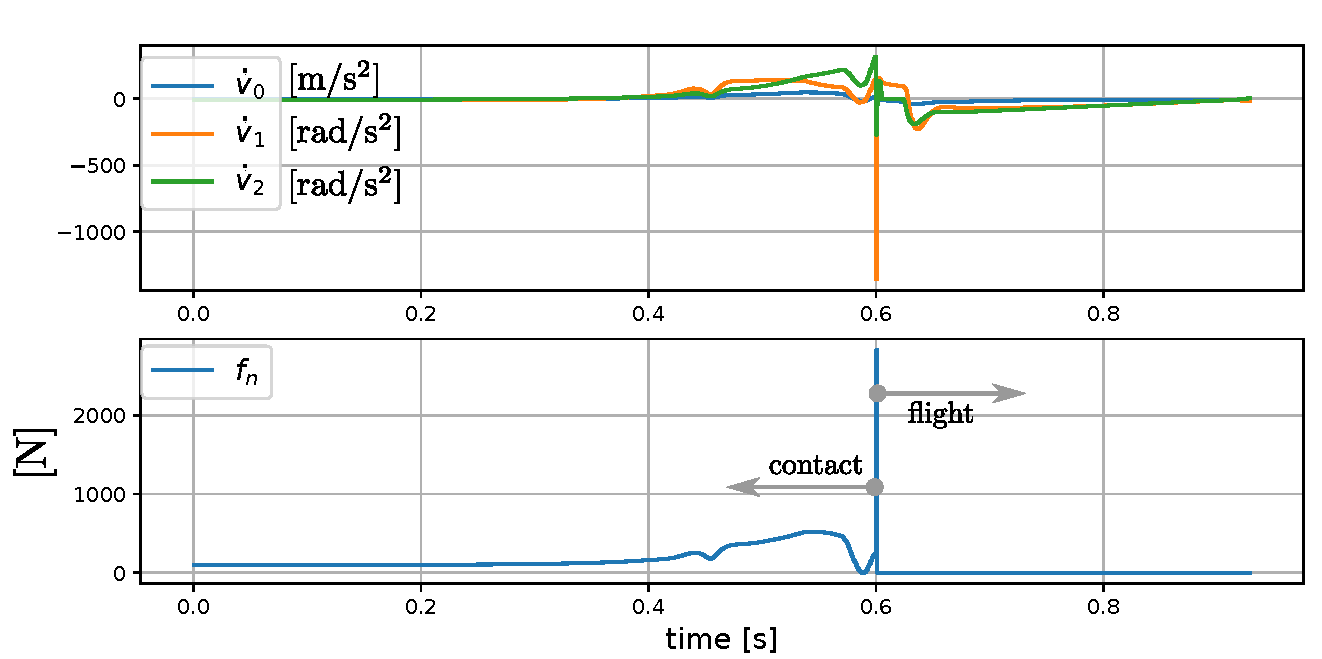
\includegraphics[width=1\columnwidth]{images/inv_dyn_caveat.pdf}
    \caption{Joint accelerations (on top) and normal component of the ground reaction force obtained for a refined take-off problem without jerk and yank minimization: the solver exploits a caveat in the inverse dynamics formulation and finds a solution which respects node constraints, but is not feasible in reality.}
    \label{fig:inv_dyn_caveat}
\end{figure}
Fig.~\ref{fig:inv_dyn_caveat} shows the results of a refined solution where the regularization costs on the jerk $\ddot{v}$ and the yank $\dot{f}$ are not employed. Looking at the picture, the solver exploits a caveat in the inverse dynamics-based formulation and produces an impulse of $f$ at the takeoff-instant without violating the inverse dynamics on the nodes. It does so by compensating with corresponding impulses of $\dot{v}$. This acceleration and ground reaction forces are however not feasible in reality, and this could be checked by looking at the dynamics residuals obtained by re-sampling the refined trajectory at a higher rate.
This shows how with the inverse dynamics-based formulation applied to highly dynamic TO needs to be complemented with suitable regularization of the jerk $\dot{v}$ and $\dot{f}$ to function properly.
\subsection{Landing phase: impact dynamics modeling}\label{subsec:impact_min}
\begin{figure}[t]
    \centering
    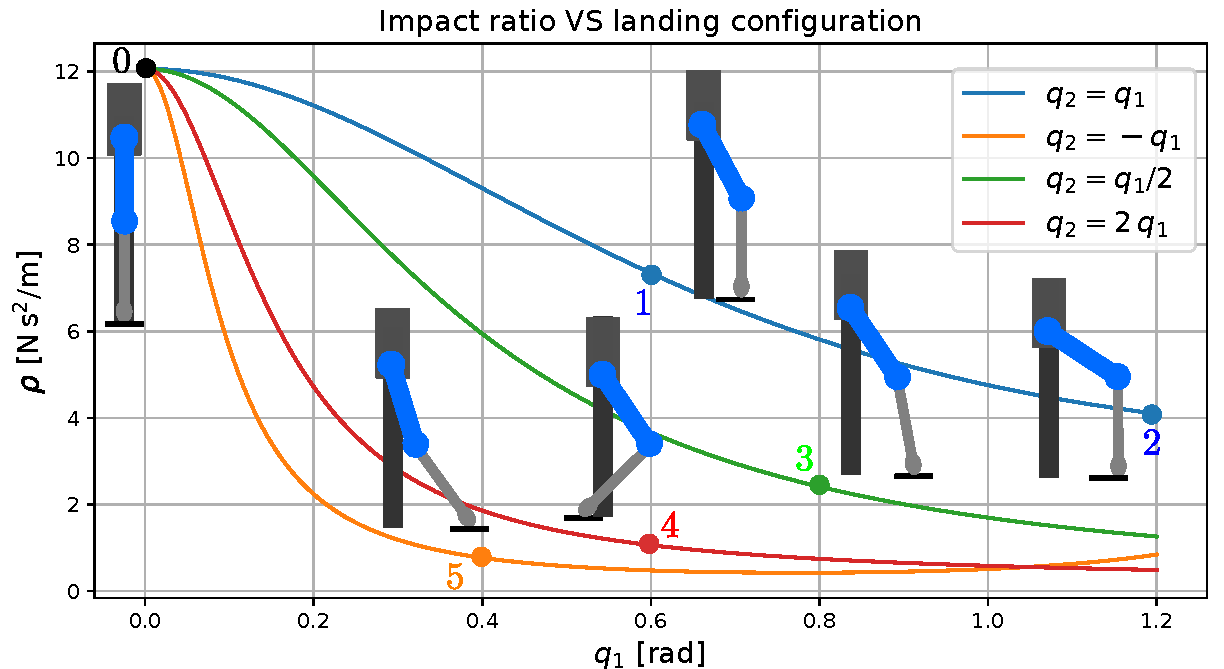
\includegraphics[width=1\columnwidth]{images/impact_ratio.pdf}
    \caption{Depending on the landing configuration, the impact felt by the robot at the ground can vary greatly. In this figure, we show how the modulus of the impact ratio $\rho$ changes with the landing configuration, which is described by the two joint variables $q_1$ and $q_2$. We specifically highlight 6 representative configurations, which are shown on top of the impact curves.}
    \label{fig:impact_ratio}
\end{figure}
After the apex of the flight phase, the leg will make contact with the ground. Under the usual assumption that the impact duration is negligible with respect to the time scale over which the body dynamics evolves, it is possible to integrate~\eqref{eq:rigid_body_dyn} over the impact instant to obtain the so called \textit{impact dynamics}~\cite{impact_dyn::walker1990use}:
\begin{equation}
    \label{eq:impact_dyn}
B(\hat{q})\,\left[v_{+} - v_{-}\right] = J^{T}(\hat{q})\,\hat{f}
\end{equation}
where $\hat{q}$ is the impact configuration of the robot, $v^{+}$ and $v^{-}$ are the post-impact and pre-impact generalized velocities of the system and $\hat{f}$ is the impact impulse, defined as the integral of the impact force during the impact interval.
The forward kinematics continues to be valid at the impact instant, so we can write
\begin{equation}\label{eq:imp_forw_dyn}
    J\,\left( v^{+} - v^{-} \right) = \dot{\chi}_{\mathrm{tip}}^{+} - \dot{\chi}_{\mathrm{tip}}^{-}
\end{equation}
where the explicit dependence upon $\hat{q}$ is dropped for simplicity and $\dot{\chi}_{\mathrm{tip}}$ is the cartesian velocity of the end-effector. 
Looking at equations~\eqref{eq:impact_dyn},~\eqref{eq:imp_forw_dyn} we see that the result of the impulse $\hat{f}$ is to produce a step in the joint velocities $v$ which, in turn, will produce a step in the end-effector velocity. 

Let us look at the energetic aspect of the impact, which is particularly relevant for our case study. The variation of kinetic energy right before and after the impact is given by the simple analytical relationship
\begin{dmath}\label{eq:delta_e_k}
    \Delta E_k = E_k^{+} - E_k^{-} = \dfrac{1}{2}\,\left({v^{+}}^T\,B\,v^{+} - {v^{-}}^T\,B\,v^{-}\right)
\end{dmath}
From~\eqref{eq:impact_dyn}, exploiting the non-singularity of $B$, we can write
\begin{equation}\label{eq:v_plus}
v^+ = B^{-1}\,J^T\,\hat{f} + v^{-}
\end{equation}
where we recall that $B$ is the generalized inertia matrix of the system~\eqref{eq:rigid_body_dyn}.
Substituting~\eqref{eq:v_plus} into~\eqref{eq:delta_e_k} and~\eqref{eq:imp_forw_dyn}, after a little rearranging, we can obtain the alternative expression
\begin{dmath}\label{eq:delta_e_k_altern}
    \Delta E_k = \dfrac{1}{2}\,\hat{f}^T\,\left(\dot{\chi}_{\mathrm{tip}}^{+} + \dot{\chi}_{\mathrm{tip}}^{-}\right)
\end{dmath}
From~\eqref{eq:delta_e_k} it is clear that, in general, energy is not conserved at the impact. As a simplification, we assume an inelastic impact with the ground (which is a good approximation for the setup shown in Fig.~\ref{fig:jumping_sequence}) and the velocity of the actuated joints to be negligible w.r.t. the linear guide velocity. This second assumption was successfully verified both in simulation and on the hardware over several jumping tests. With these premises, we can write a simplified version of~\eqref{eq:imp_forw_dyn} and~\eqref{eq:delta_e_k} for our specific case as
\begin{dmath}\label{eq:imp_forw_dyn_simpl}
    J\, v^{+} - J\, v^{-}_{*} = - \dot{\chi}_{\mathrm{tip}}^{-}
\end{dmath}
and 
\begin{dmath}\label{eq:delta_e_k_simpl}
    \Delta E_k = \dfrac{1}{2}\,\hat{f}^T\, \dot{\chi}_{\mathrm{tip}}^{-}
\end{dmath}
with 
\begin{equation} \label{eq:chi_dot_simpl}
    \dot{\chi}_{\mathrm{tip}}^{-} = \left[0, 0, 
v_{\mathrm{fall}}\right]
\end{equation}
and 
\begin{equation} \label{eq:v_m_star}
    v^{-}_{*} = \left[v_{\mathrm{fall}, 0, 0}\right]
\end{equation}
where $v_{\mathrm{fall}}$ is the vertical component of the velocity vector right before the impact.
Furthermore, we can also speculate, being the fall vertical, that most of the impulse will be concentrated on the vertical component of $\hat{f}$. As a consequence, 
\begin{equation}\label{eq:f_hat_simpl}
    \hat{f} = \begin{bmatrix}
0\\
0\\
\hat{f}_{n}
\end{bmatrix}
\end{equation}
and we can therefore conclude that, since $v_{\mathrm{fall}} \leq 0$ and $f_n > 0$ for a vertical fall, $\Delta E_{k} \leq 0$. 
Under our assumptions of inelastic and vertical impact, it is possible to combine the impact equations and arrive, after a bit of manipulation, to the following relationship between the normal component of the impact impulse and the pre-impact velocity~\cite{impact_dyn::tassi2022impact}:
\begin{equation}\label{eq:impact_ratio}
    \rho \coloneqq \dfrac{\hat{f}_n}{v_{\mathrm{fall}}} = -\dfrac{1}{\Lambda^{-1}_{2,2}(\hat{q}_1, \hat{q}_2)}
\end{equation}
to which, from now on, we will refer to as the \enquote{impact ratio}. $\Lambda^{-1}_{2,2}$ is the third element on the diagonal of the inverse cartesian inertia matrix $\Lambda^{-1} = J\,B^{-1}\,J^{T}\in\mathbb{R}^{3\times3}$. For our simple case in which the floating joint can only move vertically, $\rho$ only depends on the configuration of the leg at the impact $\left[\hat{q}_1,\hat{q}_2 \right]$.
Since we cannot know exactly when the impact will happen, $v_{\mathrm{fall}}$ cannot be used to reduce the dissipation of kinetic energy. The only option is to reduce $\hat{f}$ or, equivalently, $\rho$, which we know will depend on the landing configuration. 
Exploiting the simplicity of~\eqref{eq:impact_ratio}, we can have a quantitative glimpse at how the impact varies depending on the landing configuration. This is exactly what is shown in Fig.~\ref{fig:impact_ratio}. Most notably, the configuration n.$0$ is the absolute worst in terms of impact: all the kinetic energy is dissipated at the impact through the ground and, more importantly, through the robot itself. As a consequence, without choosing properly the landing configuration, we could potentially endanger the mechanical integrity of the robot and drastically reduce the energy available for regeneration during the braking phase.
\subsection{Landing phase: energy regeneration}\label{subsec:energy_reg}
\begin{figure}[t]
    \centering
    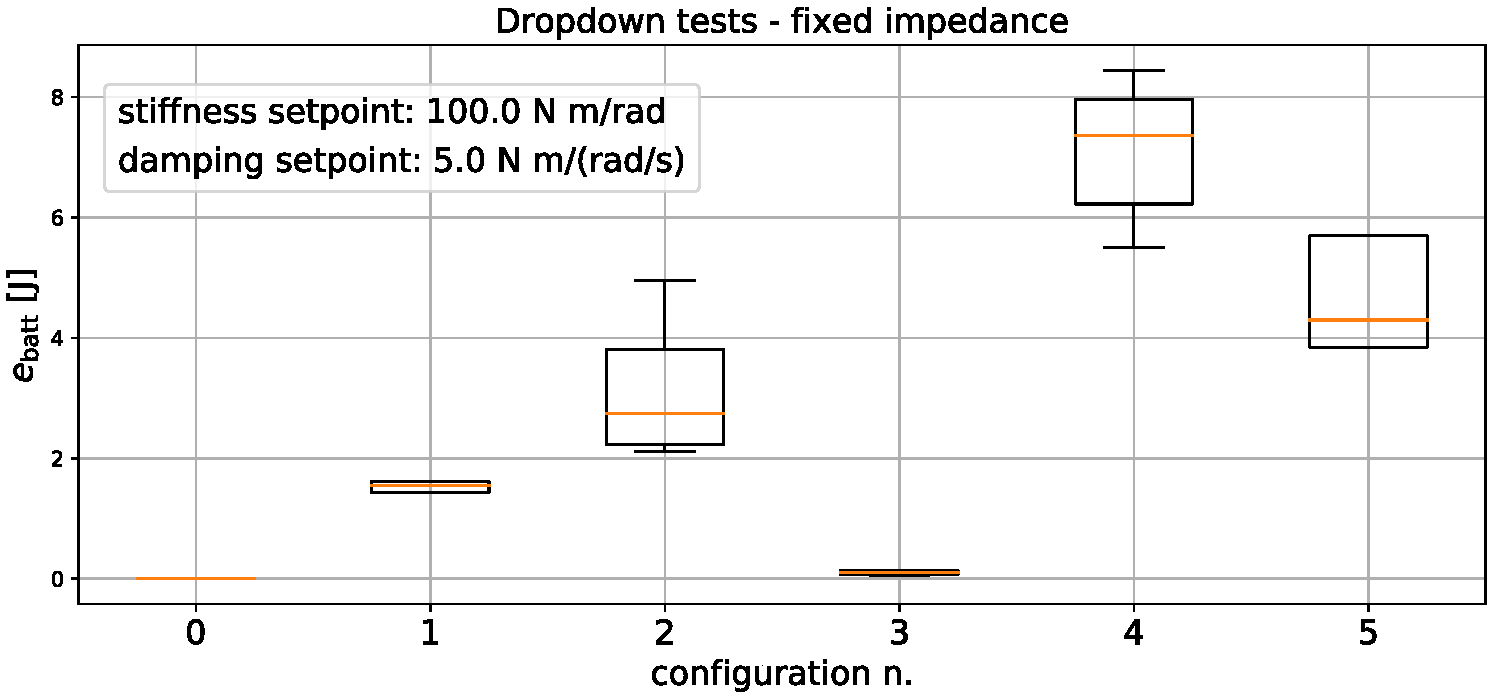
\includegraphics[width=1\columnwidth]{images/dropdown_const_imp.pdf}
    \caption{Results of the dropdown tests performed in simulation, with fixed joint impedance. The leg is dropped from an height (of the tip w.r.t. to the ground) of $0.5~\mathrm{m}$ multiple times with 6 different touchdown configurations chosen manually on the curve~\ref{fig:impact_ratio} (the same shown in Fig.~\ref{fig:impact_ratio}). At each touchdown, the regenerative energy flow $e_{\mathrm{reg}}$ towards the power source is monitored using the model~\eqref{eq:energy_flow}. The results indicate that not all configurations with low impact are equivalently suitable for energy recuperation.}
    \label{fig:fixed_imp_reg_energy}
\end{figure}
\begin{figure}[t]
    \centering
    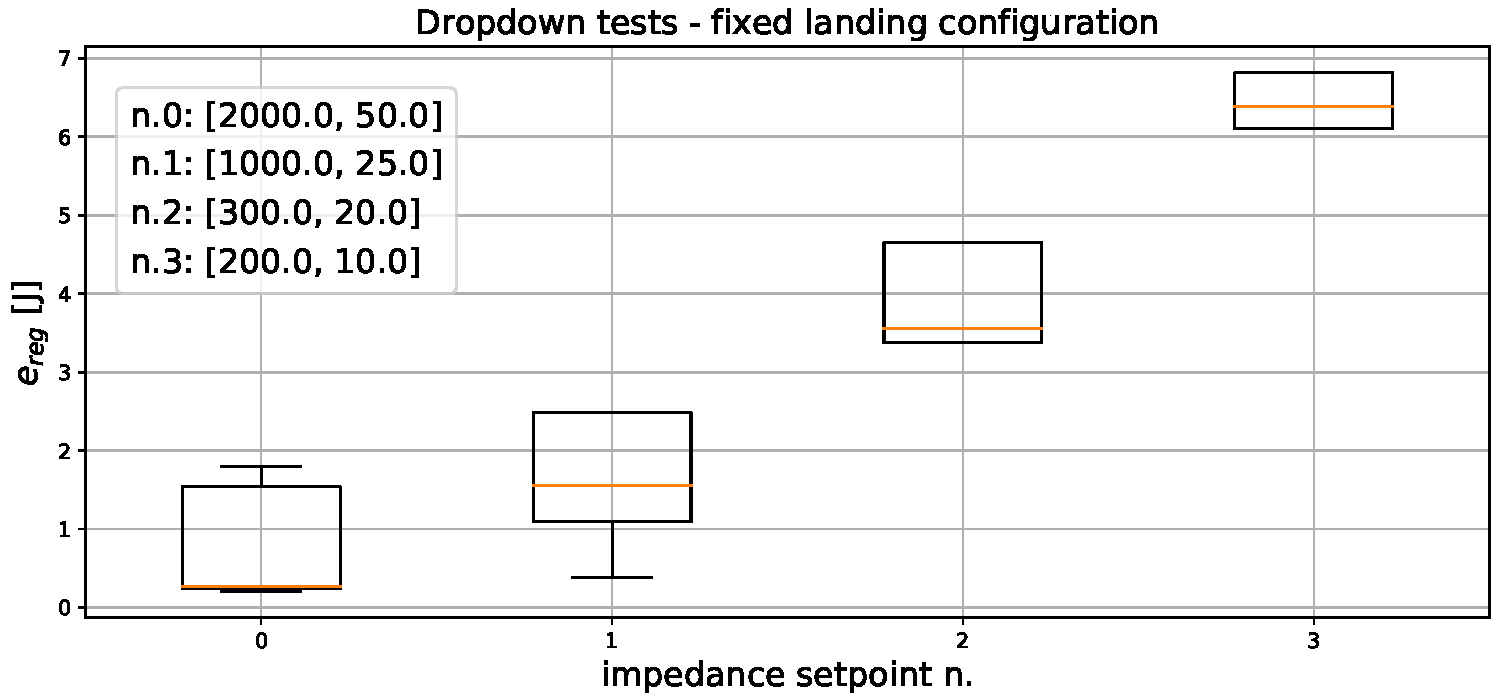
\includegraphics[width=1\columnwidth]{images/dropdown_const_landing.pdf}
    \caption{Results of the dropdown tests performed in simulation, with the landing configuration fixed to the n.~$4$ (shown in Fig.~\ref{fig:impact_ratio}). The leg is dropped from an height (of the tip w.r.t. to the ground) of $0.5~\mathrm{m}$ multiple times with 4 different joint impedance setpoints, shown at the top left of the figure (stiffness and damping setpoints, respectively). At each touchdown, the regenerative energy flow $e_{\mathrm{reg}}$ towards the power source is monitored using the energy model~\eqref{eq:energy_flow}. The results confirm that landing with stiff joints greatly diminishes the amount of energy recovered. On the contrary landing with \enquote{soft} joints diminishes the joule losses inside the actuators, due to the lower required braking torques.}
    \label{fig:fixed_conf_reg_energy}
\end{figure}

In Section~\ref{sec:prb_def} we have already qualitatively highlighted how during the braking phase it is possible to recover some of the post-impact residual energy. Here we briefly outline the formulation of a simple and effective model of the energy flow from the power source (in our case a battery) and the actuators, which will be employed in the braking TO problem outlined in the upcoming Section~\ref{subsec:energy_rec_opt}. 

When performing Field Oriented Control on BLDC motors (like in our case), it is possible to write the power balance from the battery towards the actuators in the so called \textit{qd0} reference frame employing the Park transform~\cite{foc::krause2013analysis} as 
\begin{equation}\label{eq:power_balance}
    p_{\mathrm{batt}} = - \dfrac{3}{2}\,\left(R\,i_{q}^2 + L_q\,i_{q}\,\dfrac{d}{dt}\,i_q\,\right) - K_t\,i_q\,v_m
\end{equation}
where $R$ and $L_q$ are the phase resistance and quadrature inductance of the motors and $v_m$ is the rotor velocity. The relationship, for simplicity, is shown for a single actuator. Equation~\eqref{eq:power_balance} can be integrated over an arbitrary interval of time to obtain the energy flow as
\begin{dmath} \label{eq:energy_flow}
e_{\mathrm{batt}}(t) = e_{\mathrm{batt}}(t_0)- \dfrac{3}{2}\,R\,\int_{t_0}^{t}\,i_{q}^2\,d\tau\,- \dfrac{3}{4}\,L_q\,\left[i_q^2(t) - i_q^2(t_0)\right]\,-\,K_t\,\int_{t_0}^{t}\,i_q\,v_{m}\,d\tau
\end{dmath}\vspace{-0.2cm}
Inside~\eqref{eq:energy_flow} we can distinguish, in this order, the initial energy level of the battery, the dissipative joule losses, a conservative term representing the energy stored inside the motor phases and the mechanical energy at the motor rotor. For our purposes, the inductive term in~\eqref{eq:energy_flow}, which is conservative and also weighted by $L_q$ (usually in the order of $\mu\,\mathrm{H}$), can be neglected. 

Figures~\ref{fig:fixed_imp_reg_energy} and~\ref{fig:fixed_conf_reg_energy} report data from two series of dropdown tests performed in simulation while monitoring the energy flow with~\eqref{eq:energy_flow}. 
%The leg, while being controlled by a joint-space impedance control, is dropped from an height on $0.5\mathrm{m}$ multiple times with different configurations and different joint impedance setpoints. 
After each touchdown, the energy recovered is evaluated using~\eqref{eq:energy_flow}. The results show that not all low-impact configurations are suitable for energy regeneration and that the amount of recovered energy is indeed also influenced greatly by the employed joint impedance setpoints. 
\begin{figure}[h]
    \centering
    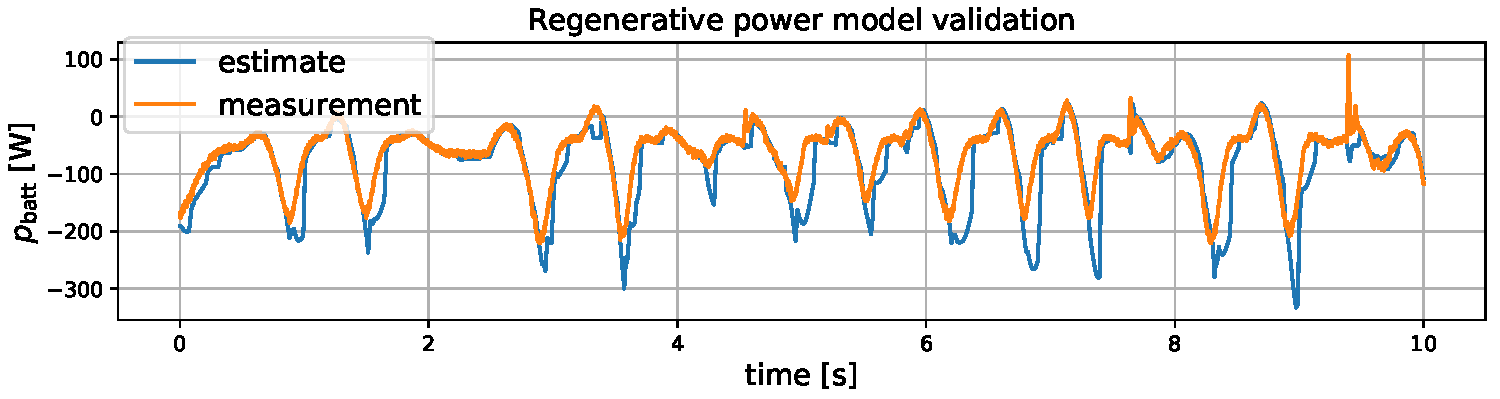
\includegraphics[width=1.0\columnwidth]{images/reg_pow_tracking.pdf}
    \caption{Validation of the model of the power flow model~\eqref{eq:power_balance}: the leg stands on the ground with low-joint impedance and an vertical oscillating force is applied to the base link. Looking at the plot, we can confirm that the model is indeed accurate in predicting the power flow of our setup.}
    \label{fig:reg_pow_model_tracking}
\end{figure}
The model~\eqref{eq:power_balance} was also successfully validated on the real hardware by employing a suitable power sensing setup. The results of the validation are shown and briefly discusses in Fig.~\ref{fig:reg_pow_model_tracking}. 
\subsection{Post-impact optimization: minimizing impact impulse and maximizing energy recovery}\label{subsec:energy_rec_opt}
Motivated by the results shown in Fig~\ref{fig:fixed_conf_reg_energy} and~\ref{fig:fixed_imp_reg_energy} and~\ref{fig:impact_ratio}, we formulate a suitable TO to jointly address the impact and power regeneration during the braking phases. As done in Sec~\ref{subsec:takeoff_opt} we employ an inverse dynamics-based formulation. In this case, the running cost takes the form
\begin{dmath}\label{eq:takeoff_running_cost_braking}
    \ell_{b}(x_b, u_b) = \ell_{p_{\mathrm{batt}}} + \ell_f + \ell_{\dot{v}}
\end{dmath}
where\vspace{-0.5cm}
\begin{eqnarray}
    x_b = \left[q,\,v\right]\\
    u_b = \left[\dot{v},\,f\right]
\end{eqnarray}
and $\ell_f$ and $\ell_{\dot{v}}$ are simple weighted quadratic regularizations on the inputs. In this case, being the braking a less dynamic phase than the take-off, we don't employ the additional regularization terms on the $\ddot{v}$ and $\dot{f}$ (see Sec.~\ref{subsec:takeoff_opt}). The weighted stage cost $\ell_{p_{\mathrm{batt}}}$ is build using directly $- p_{\mathrm{batt}}$~\eqref{eq:power_balance} and neglecting the inductive term. 
Differently from before, we formulate the problem with a fixed phase duration $T_f$ and impose the impact dynamics laws of Section~\ref{subsec:impact_min} only at the initial instant of the optimization horizon, where $v^{-}$~\eqref{eq:impact_dyn} assumes the role of a parameter of the problem. To encourage impact mitigation, we use a weighted initial cost $\ell_{\Delta E_k}^{I}$, based directly on~\eqref{eq:delta_e_k_altern}. 
%We furthermore use a simple weighted quadratic terminal cost $\ell_{v}^F$ to promote low velocities at the end of the horizon (the leg needs to break).
% \begin{eqnarray}\label{eq:reg_v}
%     % &\ell_{v, i} = \dfrac{1}{v(0)^T\,v(0) + \epsilon}\\
%     &\ell_{v, f} = v^T(T_f)\,v(T_{f})
% \end{eqnarray}
% The first term helps the solver not to get stuck in the local minima of the straight leg landing configuration n.$[0]$: looking at Figure~\ref{fig:impact_ratio}, the slope of the impact curve near the origin is small, which could cause slow convergence issues. The second term $\ell_{\dot{v}, f}$ is a simple quadratic cost to promote low velocities at the end of the horizon (the leg needs to break).
Once again, we employ the ground contact and force constraints ~\eqref{eq:tip_on_ground},~\eqref{eq:f_positive}, this time on the whole TO horizon. More importantly, we impose a joint impedance controller with
\begin{eqnarray}\label{eq:imp_cntrl}
    \tau_{l} - K_p\,\circ\,\left(q_{l} - \hat{q}\right) - K_d\,\circ\,\left(\dot{q}_{l} - 0 \right)= 0
\end{eqnarray}
where $\tau_{l}$, $q_{l}$, $\dot{q}_{l}$ refer to the actuated joint only, $K_p\in\mathbb{R}^{2}$ and $K_d\in\mathbb{R}^{2}$ are, respectively, stiffness and impedance gain vectors, which are to be optimized and $\hat{q}$ is the reference configuration for the impedance controller, which is kept constant through the horizon and equal to the landing configuration. The symbol $\circ$ is used to indicate the element-wise product between the operands.
Our final braking problem takes the form
\begin{subequations}\label{eq::braking_opt_prb}
	\begin{dmath}
		\min_{W_{b}}~L_{b}\left(W_{b}\right)
	\end{dmath}
	\centering\text{subject to}
	\begin{eqnarray}
	&\text{rigid body dynamics}~\eqref{eq:rigid_body_dyn}\\
    &\text{foot tip contact}~\eqref{eq:tip_on_ground},~\eqref{eq:f_positive}~\text{up to}~T_f\\
    &\text{joint impedance control}~ \eqref{eq:imp_cntrl} \\
    &\text{torque limits}~\eqref{eq:tau_lims}\\
    &\text{impact dynamics}~\eqref{eq:impact_dyn};~t = 0\\
    &\text{post-impact velocity:}~v^{+} = v;~t = 0\\
    &\text{landing configuration: }~q = \hat{q};~t=0\\
    &\text{joint position and velocity ranges}	\end{eqnarray}
\end{subequations}
where
\begin{dmath}
    W_{b} = \left[x_b,\,u_b,\,K_p,\,K_d,\,\hat{q}\right]
\end{dmath}
are our optimization variables and 
\begin{dmath}\label{eq:takeoff_opt_L_b}
    L_{b} \left( W_b\right) = \ell_{\Delta E_k}^{I} + \int_{0}^{T_f}\,\ell_{b}(\tau)\,d\tau
%     + \ell_{v}^F
\end{dmath}
is the employed cost function.
% It should be noted that we could have inverted~\eqref{eq:impact_dyn} and obtained analytical expressions for the relationships between $v^{+} - v^{-}$ and $i$ or $\chi_{\mathrm{tip}}^{+} - \chi_{\mathrm{tip}}^{-}$ and $i$ as done in~\cite{impact_dyn::walker1994impact}, but this would require the introduction of the well-known \textit{cartesian inertia matrix} $\Lambda\,\coloneqq \left(J\,B^{-1}\,J^{T}\right)$. This in turn, would need the computation of $B^{-1}$, which would reintroduce the issues related to forward dynamics formulations~\cite{to::ferrolho2021inverse}. 
The only parameter over which~\eqref{eq::braking_opt_prb} depends is the pre-impact velocity $v^{-}$ (through the impact dynamics constraint~\eqref{eq:impact_dyn}) which, under the simplifications outlined in Sec.~\ref{subsec:impact_min}, can be approximated with~\eqref{eq:v_m_star}. Given the apex tip height $h_{\mathrm{tip}}$ provided by the solution of~problem~\eqref{eq::takeoff_opt_prb}, we can compute a reasonable estimate for $v^{-}$ as $[-\sqrt{2\,g\,h_{\mathrm{tip}}},~0,~0]$, where $g$ is the acceleration of gravity.
